\documentclass[12pt]{article}

\usepackage{algorithm}
\usepackage{algorithmicx}
\usepackage{algpseudocode}
\usepackage{amsmath}
\usepackage{amsthm}
\usepackage{tikz}
\usetikzlibrary{arrows,automata}

\title{EECS 477 HW3}
\author{Andrew Mason}

\begin{document}
\maketitle

\begin{enumerate}
    % #1
    \item
        I originally thought to model this as a variation of the matrix
        rounding problem discussed in class, but this has the unfortunate
        result of actually maximizing the number of nurses assigned to each
        shift/department pair.

        Instead, if we start by assigning the maximum number of nurses allowed
        to each shift/department pair, we can formulate another variation of
        the matrix rounding problem which attempts to maximize the number of
        nurses witheld from each shift/department pair. The edges incident on
        the ``matrix nodes'' (the nodes representing each shift/department
        pair) each have $l_{ij},u_{ij}=0,d$, where $d$ is the difference
        between the lower and upper bounds for that node in the original
        matrix. The column nodes then have $l_{ij},u_{ij}=0, d_c$, where $d_c$
        is the difference between the column lower bound in the original
        matrix, and the sum of the upper bounds for each matrix node in the
        original matrix. The row nodes similarly have $l_{ij},u_{ij}=0,d_r$.

        So, our network looks like:
        \begin{center}
            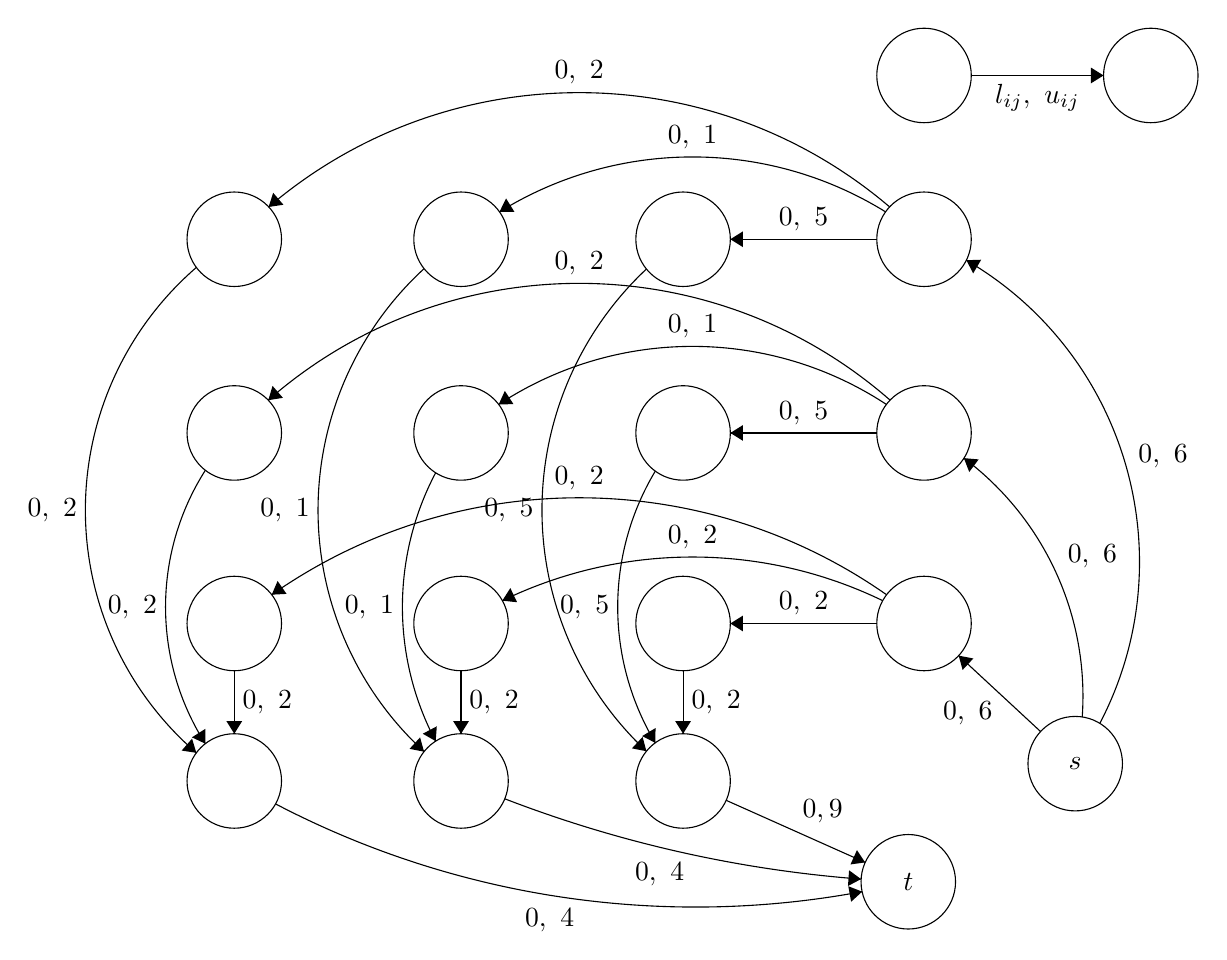
\begin{tikzpicture}[scale=0.2]
                \tikzstyle{every node}+=[inner sep=0pt]
                \draw [black] (56.5,-4) circle (3);
                \draw [black] (70.9,-4) circle (3);
                \draw [black] (12.7,-14.4) circle (3);
                \draw [black] (27.1,-14.4) circle (3);
                \draw [black] (41.2,-14.4) circle (3);
                \draw [black] (56.5,-14.4) circle (3);
                \draw [black] (12.7,-26.7) circle (3);
                \draw [black] (27.1,-26.7) circle (3);
                \draw [black] (41.2,-26.7) circle (3);
                \draw [black] (56.5,-26.7) circle (3);
                \draw [black] (12.7,-38.8) circle (3);
                \draw [black] (27.1,-38.8) circle (3);
                \draw [black] (41.2,-38.8) circle (3);
                \draw [black] (56.5,-38.8) circle (3);
                \draw [black] (12.7,-48.8) circle (3);
                \draw [black] (27.1,-48.8) circle (3);
                \draw [black] (41.2,-48.8) circle (3);
                \draw [black] (55.5,-55.2) circle (3);
                \draw (55.5,-55.2) node {$t$};
                \draw [black] (66.1,-47.7) circle (3);
                \draw (66.1,-47.7) node {$s$};
                \draw [black] (59.5,-4) -- (67.9,-4);
                \fill [black] (67.9,-4) -- (67.1,-3.5) -- (67.1,-4.5);
                \draw (63.7,-4.5) node [below] {$l_{ij},\mbox{ }u_{ij}$};
                \draw [black] (59.185,-15.733) arc (59.72274:-27.55944:22.175);
                \fill [black] (59.19,-15.73) -- (59.62,-16.57) -- (60.13,-15.7);
                \draw (70.08,-28.17) node [right] {$0,\mbox{ }6$};
                \draw [black] (59.033,-28.302) arc (53.13091:-3.99657:18.896);
                \fill [black] (59.03,-28.3) -- (59.37,-29.18) -- (59.97,-28.38);
                \draw (65.6,-34.54) node [right] {$0,\mbox{ }6$};
                \draw [black] (63.9,-45.66) -- (58.7,-40.84);
                \fill [black] (58.7,-40.84) -- (58.95,-41.75) -- (59.63,-41.02);
                \draw (59.28,-43.74) node [below] {$0,\mbox{ }6$};
                \draw [black] (53.5,-14.4) -- (44.2,-14.4);
                \fill [black] (44.2,-14.4) -- (45,-14.9) -- (45,-13.9);
                \draw (48.85,-13.9) node [above] {$0,\mbox{ }5$};
                \draw [black] (29.542,-12.661) arc (121.76626:58.23374:23.284);
                \fill [black] (29.54,-12.66) -- (30.49,-12.66) -- (29.96,-11.81);
                \draw (41.8,-8.67) node [above] {$0,\mbox{ }1$};
                \draw [black] (14.885,-12.346) arc (130.41235:49.58765:30.412);
                \fill [black] (14.88,-12.35) -- (15.82,-12.21) -- (15.17,-11.45);
                \draw (34.6,-4.59) node [above] {$0,\mbox{ }2$};
                \draw [black] (53.5,-26.7) -- (44.2,-26.7);
                \fill [black] (44.2,-26.7) -- (45,-27.2) -- (45,-26.2);
                \draw (48.85,-26.2) node [above] {$0,\mbox{ }5$};
                \draw [black] (29.489,-24.889) arc (123.33513:56.66487:22.403);
                \fill [black] (29.49,-24.89) -- (30.43,-24.87) -- (29.88,-24.03);
                \draw (41.8,-20.7) node [above] {$0,\mbox{ }1$};
                \draw [black] (14.856,-24.615) arc (131.17311:48.82689:29.991);
                \fill [black] (14.86,-24.62) -- (15.79,-24.47) -- (15.13,-23.71);
                \draw (34.6,-16.7) node [above] {$0,\mbox{ }2$};
                \draw [black] (53.5,-38.8) -- (44.2,-38.8);
                \fill [black] (44.2,-38.8) -- (45,-39.3) -- (45,-38.3);
                \draw (48.85,-38.3) node [above] {$0,\mbox{ }2$};
                \draw [black] (29.724,-37.349) arc (115.84349:64.15651:27.703);
                \fill [black] (29.72,-37.35) -- (30.66,-37.45) -- (30.23,-36.55);
                \draw (41.8,-34.08) node [above] {$0,\mbox{ }2$};
                \draw [black] (15.078,-36.973) arc (125.01248:54.98752:34.025);
                \fill [black] (15.08,-36.97) -- (16.02,-36.92) -- (15.45,-36.1);
                \draw (34.6,-30.32) node [above] {$0,\mbox{ }2$};
                \draw [black] (12.7,-41.8) -- (12.7,-45.8);
                \fill [black] (12.7,-45.8) -- (13.2,-45) -- (12.2,-45);
                \draw (13.2,-43.8) node [right] {$0,\mbox{ }2$};
                \draw [black] (27.1,-41.8) -- (27.1,-45.8);
                \fill [black] (27.1,-45.8) -- (27.6,-45) -- (26.6,-45);
                \draw (27.6,-43.8) node [right] {$0,\mbox{ }2$};
                \draw [black] (41.2,-41.8) -- (41.2,-45.8);
                \fill [black] (41.2,-45.8) -- (41.7,-45) -- (40.7,-45);
                \draw (41.7,-43.8) node [right] {$0,\mbox{ }2$};
                \draw [black] (43.94,-50.03) -- (52.76,-53.97);
                \fill [black] (52.76,-53.97) -- (52.24,-53.19) -- (51.83,-54.1);
                \draw (50.06,-51.48) node [above] {$0,9$};
                \draw [black] (52.505,-55.031) arc (-94.31889:-111.08028:79.568);
                \fill [black] (52.5,-55.03) -- (51.74,-54.47) -- (51.67,-55.47);
                \draw (39.71,-53.97) node [below] {$0,\mbox{ }4$};
                \draw [black] (52.567,-55.827) arc (-79.41981:-117.58934:57.589);
                \fill [black] (52.57,-55.83) -- (51.69,-55.48) -- (51.87,-56.47);
                \draw (32.73,-56.86) node [below] {$0,\mbox{ }4$};
                \draw [black] (10.864,-46.433) arc (-147.51999:-212.48001:16.169);
                \fill [black] (10.86,-46.43) -- (10.86,-45.49) -- (10.01,-46.03);
                \draw (7.83,-37.75) node [left] {$0,\mbox{ }2$};
                \draw [black] (25.488,-46.274) arc (-152.16764:-207.83236:18.257);
                \fill [black] (25.49,-46.27) -- (25.56,-45.33) -- (24.67,-45.8);
                \draw (22.88,-37.75) node [left] {$0,\mbox{ }1$};
                \draw [black] (39.436,-46.378) arc (-149.04755:-210.95245:16.776);
                \fill [black] (39.44,-46.38) -- (39.45,-45.44) -- (38.6,-45.95);
                \draw (36.55,-37.75) node [left] {$0,\mbox{ }5$};
                \draw [black] (10.294,-47.012) arc (-130.83998:-229.16002:20.372);
                \fill [black] (10.29,-47.01) -- (10.02,-46.11) -- (9.36,-46.87);
                \draw (2.74,-31.6) node [left] {$0,\mbox{ }2$};
                \draw [black] (24.753,-46.936) arc (-132.58201:-227.41799:20.828);
                \fill [black] (24.75,-46.94) -- (24.5,-46.03) -- (23.83,-46.76);
                \draw (17.52,-31.6) node [left] {$0,\mbox{ }1$};
                \draw [black] (38.872,-46.911) arc (-133.15246:-226.84754:20.988);
                \fill [black] (38.87,-46.91) -- (38.63,-46) -- (37.95,-46.73);
                \draw (31.74,-31.6) node [left] {$0,\mbox{ }5$};
            \end{tikzpicture}
        \end{center}

        And this can now be solved by max flow.\\
    % #2
    \item
        For each region $x_j$, create an intermediate node. Put an arc from
        each skilled contractor $c_i$ to this node, with cost $c_{ij}$, lower
        bound 0, and upper bound $\infty$. Then put a single arc going from
        this intermediate node to $x_j$, with cost 0, lower bound 1 and upper
        bound $\infty$. This ensures that all regions get at least one skilled
        contractor. Then, for each unskilled contractor, put an arc directly
        from the contractor to the region, with cost $c_{ij}$, lower bound 0
        and upper bound $\infty$. Next, assign a supply of $u_i$ to each
        contractor $c_i$, and a demand of $r_j$ to each region $x_j$. Finally,
        create a sink with a demand $\sum_{i}u_i - \sum_jr_j$ and place an arc
        going from each contractor to the sink. Each of these arcs should have
        cost 0, lower bound 0, upper bound $\infty$. This will capture any
        extra teams that did not need to be assigned to a region. I should also
        add that the intermediate nodes discussed above are transhipment nodes,
        so their supplies should each be 0.

        So, for a contractor problem with 3 contractors (2 skilled), and 2
        regions, we would have (note that since all upper bounds are $\infty$,
        they have been ignored):

        \begin{center}
            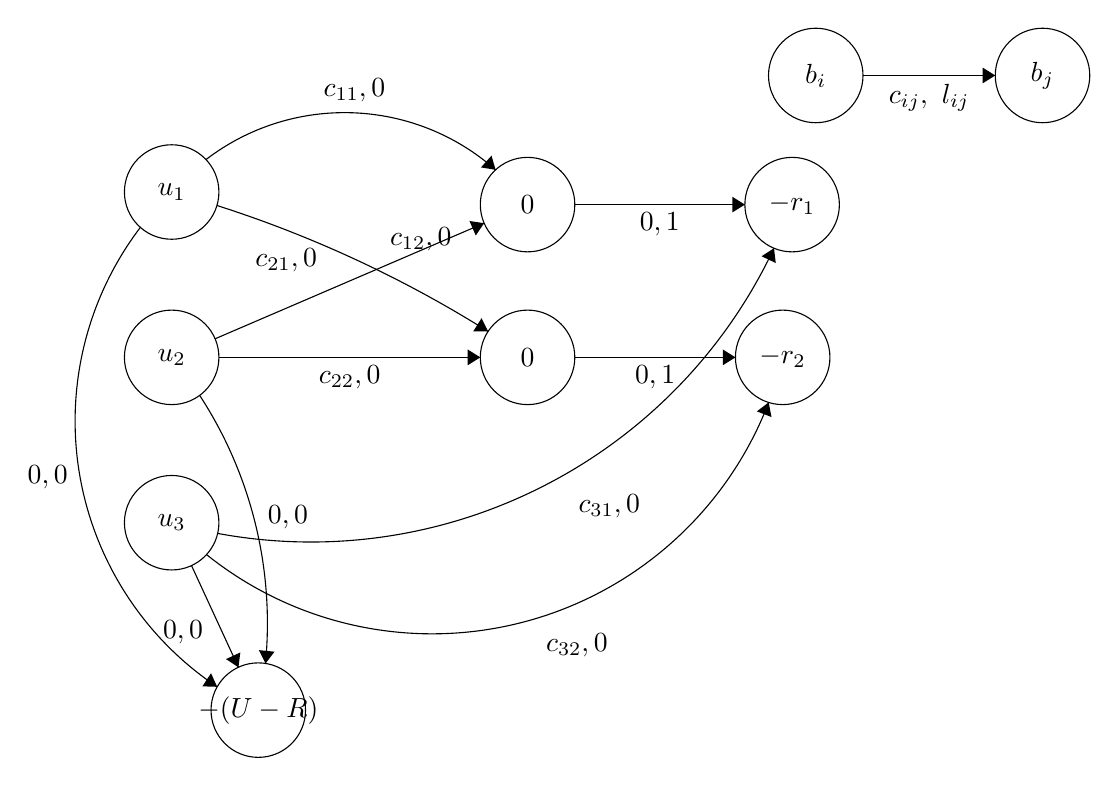
\begin{tikzpicture}[scale=0.2]
                \tikzstyle{every node}+=[inner sep=0pt]
                \draw [black] (56.5,-4) circle (3);
                \draw (56.5,-4) node {$b_i$};
                \draw [black] (70.9,-4) circle (3);
                \draw (70.9,-4) node {$b_j$};
                \draw [black] (15.6,-11.4) circle (3);
                \draw (15.6,-11.4) node {$u_1$};
                \draw [black] (15.6,-21.9) circle (3);
                \draw (15.6,-21.9) node {$u_2$};
                \draw [black] (15.6,-32.4) circle (3);
                \draw (15.6,-32.4) node {$u_3$};
                \draw [black] (55,-12.2) circle (3);
                \draw (55,-12.2) node {$-r_1$};
                \draw [black] (54.4,-21.9) circle (3);
                \draw (54.4,-21.9) node {$-r_2$};
                \draw [black] (38.2,-12.2) circle (3);
                \draw (38.2,-12.2) node {$0$};
                \draw [black] (38.2,-21.9) circle (3);
                \draw (38.2,-21.9) node {$0$};
                \draw [black] (21.1,-44.3) circle (3);
                \draw (21.1,-44.3) node {$-(U-R)$};
                \draw [black] (59.5,-4) -- (67.9,-4);
                \fill [black] (67.9,-4) -- (67.1,-3.5) -- (67.1,-4.5);
                \draw (63.7,-4.5) node [below] {$c_{ij},\mbox{ }l_{ij}$};
                \draw [black] (17.776,-9.343) arc (127.45108:48.49428:14.478);
                \fill [black] (36.17,-9.99) -- (35.91,-9.09) -- (35.24,-9.84);
                \draw (27.2,-5.73) node [above] {$c_{11},0$};
                \draw [black] (18.36,-20.72) -- (35.44,-13.38);
                \fill [black] (35.44,-13.38) -- (34.51,-13.24) -- (34.91,-14.16);
                \draw (22.87,-16.5) node [above] {$c_{21},0$};
                \draw [black] (41.2,-12.2) -- (52,-12.2);
                \fill [black] (52,-12.2) -- (51.2,-11.7) -- (51.2,-12.7);
                \draw (46.6,-12.7) node [below] {$0,1$};
                \draw [black] (18.475,-12.256) arc (72.28468:57.87599:75.688);
                \fill [black] (35.69,-20.25) -- (35.28,-19.41) -- (34.75,-20.25);
                \draw (31.42,-15.18) node [above] {$c_{12},0$};
                \draw [black] (18.6,-21.9) -- (35.2,-21.9);
                \fill [black] (35.2,-21.9) -- (34.4,-21.4) -- (34.4,-22.4);
                \draw (26.9,-22.4) node [below] {$c_{22},0$};
                \draw [black] (41.2,-21.9) -- (51.4,-21.9);
                \fill [black] (51.4,-21.9) -- (50.6,-21.4) -- (50.6,-22.4);
                \draw (46.3,-22.4) node [below] {$0,1$};
                \draw [black] (16.86,-35.12) -- (19.84,-41.58);
                \fill [black] (19.84,-41.58) -- (19.96,-40.64) -- (19.05,-41.06);
                \draw (17.63,-39.38) node [left] {$0,0$};
                \draw [black] (17.378,-24.314) arc (33.12213:-5.53163:26.481);
                \fill [black] (21.56,-41.34) -- (22.13,-40.59) -- (21.14,-40.49);
                \draw (21.68,-32.03) node [right] {$0,0$};
                \draw [black] (18.492,-42.823) arc (-123.74905:-217.26983:20.305);
                \fill [black] (18.49,-42.82) -- (18.1,-41.96) -- (17.55,-42.79);
                \draw (9.03,-29.52) node [left] {$0,0$};
                \draw [black] (53.848,-14.969) arc (-25.22653:-100.48591:32.512);
                \fill [black] (53.85,-14.97) -- (53.06,-15.48) -- (53.96,-15.91);
                \draw (43.39,-30.56) node [below] {$c_{31},0$};
                \draw [black] (53.511,-24.763) arc (-20.99749:-128.7173:22.898);
                \fill [black] (53.51,-24.76) -- (52.76,-25.33) -- (53.69,-25.69);
                \draw (41.33,-39.42) node [below] {$c_{32},0$};
            \end{tikzpicture}
        \end{center}
        where $U=\sum_iu_i$ and $R=\sum_jr_j$.

        The standard form for MCNF duality is:
        \begin{equation}
            \begin{split}
                \text{max}\ &\sum_{i\in V}b_i\pi_i - \sum_{\left(i,j\right)\in E}u_{ij}\alpha_{ij}\\
                \text{s.t.}\ &\pi_i-\pi_j-\alpha_{ij}\leq0\text{ for all i,j}\\
                &\alpha_{ij}\geq0\\
                &\pi_i\ \text{unrestricted}\\
            \end{split}
        \end{equation}

        Now, since each $u_{ij}=\infty$, all $\alpha_{ij}=0$, or the dual is
        infeasible (objective value goes to $-\infty$). So, I will simply
        ignore second summation in the objective function. The dual for the
        contractors problem is then:
        \begin{equation}
            \begin{split}
                \text{max}\ &\sum_{i\in V_C}u_i\pi_i - \sum_{j\in V_R}r_j\pi_j - (U-R)\pi_s\\
                \text{s.t.}\ &\pi_i-\pi_j-\alpha_{ij}\leq0\text{ for all i,j}\\
                &\alpha_{ij}\geq0\\
                &\pi_i\ \text{unrestricted}\\
            \end{split}
        \end{equation}
        where $V_C$ is the set of nodes that are contractors, $V_R$ is the set
        of nodes that are regions, $\pi_s$ is the node potential corresponding
        to the sink node, and $U,R$ defined as above. All of the other nodes
        have supplies and demands of 0, so they do not appear in the objective
        function.\\

        The complimentary slackness conditions are:
        \begin{itemize}
            \item $\alpha_{ij}\left(u_{ij}-x_{ij}\right)=0$
            \item $x_{ij}\left(c^\pi_{ij}+\alpha_{ij}\right)=0$
        \end{itemize}

        Since we know that all $\alpha_{ij}=0$, this actually leaves us with
        just:
        $$x_{ij}c^\pi_{ij}=0$$

        So, this tells us that for an optimal solution to the contractor
        problem, either an arc in the original network gets no flow, or the
        reduced cost for that arc is 0.\\
    % #3
    \item
    % #4
    \item Omitted.\\
    % #5
    \item
    % #6
    \item Postponed.\\
    % #7
    \item
    % #8
    \item Postponed.\\
\end{enumerate}
\end{document}
